\apendice{Documentación técnica de programación}

\section{Introducción}
En el siguiente apartado se detallarán requisitos, herramientas, pautas\ldots para trabajar con este proyecto.\\
El proyecto se puede descargar del Repositorio GitHub pulsando \href{https://github.com/jct0024/HealthApp}{aquí}.
\section{Estructura de directorios}
Los directorios siguen la siguiente estructura:
\begin{itemize}
\item Directorio: ForDevelopments
\begin{itemize}
\item Directorio: assets
\begin{itemize}
\item Manual.pdf
\item Logotipo.PNG
\item logo.ico
\item A.png
\item B.png
\item C.png
\item D.png
\item E.png
\item caraRoja.png
\item caraVerde.png
\end{itemize}
\item Directorio: Dat
\begin{itemize}
\item BaseDeDatosDeAlimentos.xlsx
\item BaseDeDatosUsuarios.xlsx
\item Historial.xlsx
\item config.txt
\item RegistroHistorial
\end{itemize}
\begin{itemize}
\item requirements.txt
\item Intructions.txt
\end{itemize}

\item AdminBase.py
\item Main.py
\item CalculosDieta.py
\item Vista.py
\end{itemize}
\item Directorio: ForUsers.
\begin{itemize}
\item Directorio: HeatlhApp (Contiene el ejecutable).
\item Manual.pdf
\item Instructions.txt
\end{itemize}
\item Directorio: Memorias
\begin{itemize}
\item Anexos.pdf
\item Memorias.pdf
\item Directorio: img (Almacenamiento de imágenes)
\item Directorio: LatEx (Memorias y anexos en LatEx.
\end{itemize}
\item Directorio: Poster (Poster del programa).
\item Directorio: Vídeos (Ayudas audivisuales para usuarios y desarrolladores).
\end{itemize}
\section{Manual del programador}
A continuación se observa una pequeña guía para preparar el entorno de programación.\\

\textbf{\textsc{Python}}\\
El lenguaje usado durante este proyecto es Python en su versión 3.7. Para ello tendrá que descargar e instalar el interprete de Python desde el siguiente enlace \href{https://www.python.org/downloads/}{Python 3.7.3}. Para su descarga se ha de pulsar el botón: \textbf{Download Python 3.7.3}\\

Se instala Anaconda (no es estrictamente necesario, pero es el sistema usado para el desarrollo del proyecto), el cual nos dará una serie de funciones y programas, además de una powershell propia, muy útiles. Link: \href{https://www.anaconda.com/distribution/}{Anaconda}.\\
Con esto, se nos instalará automáticamente tanto Spyder, como Notebook y VisualCode. Cualquiera de estos tres editores son muy potentes y funcionan a la perfección para ejecutar el proyecto (aunque se aconseja no usar NoteBook). Además esta herramienta viene con una serie de librerías principales ya instaladas que ahorran trabajo al programador.\\

En caso de no instalar anaconda, se debería instalar un editor, para su posterior ejecución. Editores recomendados para Python:
\begin{itemize}
\item PyCharm.
\item VisualCode.
\item Spyder.
\item Eclipse con IDE Python.
\end{itemize}
Recordar que si se escoge un editor que no tenga la opción de ejecutar directamente, se deberá hacer a través de la consola de comandos. Para ello vaya a la carpeta donde tenga descargado el proyecto, y en la parte superior (donde aparece la ruta del directorio) escriba cmd y se cargará la powershell desde la carpeta actual. Acto seguido escriba HealthApp.py y el programa se ejecutará para su prueba o test.\\

Las siguientes librerías son las librerías principales usadas durante el proyecto:
\begin{itemize}
\item matplotlib
\item numpy
\item pandas
\item auto-py-to-exe
\item webbrowser
\item os-win
\item Pillow
\item functools
\item xlrd
\item openpyxl
\end{itemize}
Auto-py-to-exe es una librería que sirve para crear archivos ejecutables desde un archivo con extensión ".py", sencilla de usar. Utiliza pyinstaler de manera interna y proporciona una interfaz gráfica intuitiva para crear el ejecutable. El resto de librerías son las usadas para que el programa funcione con normalidad.\\

\textbf{\textsc{Auto-py-to-exe}}\\
Para usar la aplicación auto-py-to-exe abriremos la consola de comandos con \textbf{cmd}, y escribiremos el comando \textbf{auto-py-to-exe}
\imagen{consolaAuto}{Comando para el uso de auto-py-to-exe.}
Cuando inserte ese comando se abrirá una ventana como la siguiente:
\imagen{autopy}{Pantalla de la aplicación auto-py-to-exe.}
Para su correcto uso se deberá añadir en \textbf{path file} el archivo principal (HealthApp) que ejecuta todo nuestro programa. Para evitar problemas con los archivos extra, se marcará la opción \textbf{''One Directory''}, y más adelante la opción \textbf{Windows Based (console hidden)} para evitar que se reproduzca la consola cada vez que lo ejecutemos (si deseamos depurar el programa se aconseja usar la otra opción).\\

Para terminar añadimos el icono de la aplicación en \textbf{Icon} y en \textbf{Additional Files} se elegirá la opción \textbf{add folder} y se añadirá las carpetas de "assets" y "Dat". Una vez hecho, se pulsará sobre el botón \textbf{Convert .py to .exe}. Si no hemos escogido carpeta de salida se hará sobre la carpeta propia del proyecto, y si deseamos que se cree en cualquier otra carpeta específica se deberá añadir la ruta dentro de las opciones que se encuentran en \textbf{Advanced}.\\
\textbf{\textsc{INSTALACIÓN DE LAS LIBRERÍAS}}\\
Para comodidad del desarrollador se dejará preparado el documento: \textbf{requeriments.txt} donde estarán almacenadas todas las librerías necesarias, si se desea instalar a través de este documento se ha de ejecutar el siguiente comando en la Shell: \textbf{pip3 install -r requeriments.txt}.\\

Además existirá la carpeta \textbf{ForDevelopmnet}, donde encontrará dicho archivo (requeriments.txt) y un resumen sobre como trabajar con el proyecto.\\

En caso de existir algún fallo con alguna librería, instalar manualmente la librería concreta con el comando: \textbf{pip3 install NombreLibreria}.
Una vez esté preparado el entorno de Python, se podrá pasar a la instalación del IDE.
\subsection{IDE}
En este aparado se habla de como descargar y preparar el entorno para trabajar, y de como se realizó durante estos meses.\\

\textbf{\textsc{Spyder}}\\
Si se ha realizado la correcta instalación de Anaconda, tendrá instalado este programa por defecto.
\imagen{Spyder}{Interfaz del editor Spyder para Python.}

\textbf{\textsc{Git}}\\
Sistema de control versiones seleccionado para este proyecto. El programa no está preinstalado con Windows, por lo que se deberá descargarlo e instalarlo desde el siguiente enlace: \href{https://git-scm.com/}{Git}.\\

\textbf{\textsc{GitKraken}}\\
Para una mejor gestión, se ha usado la herramienta de escritorio Gitkraken. Si se desea descargar se puede hacer entrando en \href{https://gitkraken.com/}{GitKraken}.\\
Se descarga e instala el ejecutable, y una vez abierto el programa deberá ir a \textbf{File/Clone Repo} y añadir la URL del proyecto GitHub. Una vez clonado deberá dar a la opción \textbf{Open Repo} y buscar la carpeta donde se haya descargado previamente.\\
\imagen{GitKraken}{GitKraken}

\section{Compilación, instalación y ejecución del proyecto}
Lo primero que hay que hacer es abrir el editor, en el caso de este proyecto Spyder. Una vez abierto el editor debemos abrir los archivos *.py. Para ello pulsamos en archivo -> Abrir.\\
No es necesario abrir todos los archivos, basta con abrir el archivo Main (HealthApp) para su ejecución. Pulsamos el botón \textbf{ejecutar} que se encuentra en la parte superior, como se muestra a continuación:
\imagen{Play}{Botón ejecutar de Spyder.}
Una vez pulsado, se abrirá en otra pantalla generada por Tkinter el programa principal (Imagen: \ref{fig:Inicio}).\\
\begin{figure}[htb]
\centering
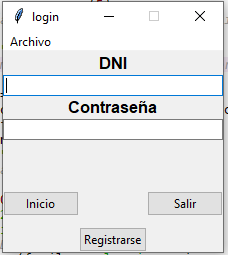
\includegraphics[scale=1]{Inicio} 
\caption{Pantalla nueva generada por la librería Tkinter (Versión 2.0)}
\label{fig:Inicio}
\end{figure}
\pagebreak

\textbf{Terminal}\\
Ante cualquier prueba que se desee realizar, aparecerá en la interfaz de Spyder la terminal. Por defecto se encuentra posicionada abajo a la derecha:
\imagen{Terminal}{Señalización de la terminal interna de Spyder.}
\section{Pruebas del sistema}
Las pruebas del sistema son para comprobar la correcta salida de información del transcurso entre Frames de manera adecuada, de la veracidad de los resultados de los cálculos internos, etcétera.
\subsection{Almacenamiento y carga de los datos}
Consisten en una serie de pruebas donde se han abordado todas las posibles combinaciones de carga y almacenamiento de los datos. Por ejemplo:
\begin{itemize}
\item Nuevo Usuario, Nuevo Alimento, Editar Usuario, Hacer selección y Refrescar selecciones, todo de manera independiente.
\item Combinaciones varias entre las opciones anterior, editando un usuario que acabo de crear, añadiendo un alimento y haciendo una selección, editando un usuario y haciendo una seleccion, etcétera. Comprobando acto seguido que se haya guardado correctamente en la base de datos.
\end{itemize}
\textbf{Problemas encontrados:}\\
Los DataFrames en ocasiones se ordenaban alfabéticamente a la hora del almacenamiento, provocando una inconsistencia de los datos con el programa. Los datos se guardan como objetos de Python en vez de como valores. Además, se tuvo que eliminar los indices de fila debido a un problema de compatibilidad en la carga de los datos en otros ordenadores.
\subsection{Navegabilidad}
Se navegó reiteradamente por la interfaz gráfica haciendo uso de todas las funciones posibles del programa, comprobando que este fuera fluido y no diera ningún tipo de problema a la hora de cambiar de Frame o generar nuevas ventanas.\\

\textbf{Observaciones:}\\
Se percibieron pequeños tiempos de espera. Los Frames son creados al inicio y mantiene su forma durante toda la navegabilidad del programa, haciéndolo una vez creado más rápido, pero dando problemas en cuanto a cambios gráficos se refiriese. Debido a la actualización de Frames por cada selección, se muestra una pequeña ralentización del programa mientras crea de nuevos los Frames.
\subsection{Algoritmos}
Se llevaron a cabo las comprobaciones necesarias para ver que el sistema de recomendación y de reparto de datos funcionara correctamente. Para ello se realizaron las siguientes pruebas:
\begin{itemize}
\item Comprobar el Cálculo TMB para personas con diferentes capacidades físicas.
\item Comprobar las recomendaciones resultantes a una serie de individuos específicos, revisando todas las opciones recomendadas.
\item Comprobar la distribución calórica de todos los tipos de dietas posibles.
\item Comprobar la correcta actualización de los datos en cuanto a la selecciones.
\end{itemize}
\textbf{Problemas encontrados:}\\
Se encontraron una serie de problemas que fueron corregidos en el acto. El sistema de recomendación fallaba ya que se quedaba con el alimento con menor diferencia, es decir, es tan mala una diferencia de 800 como de -800. Para ello se halló el valor absoluto de la fórmula.\\
Resultó que se hallaban bien los tipos de dietas pero no eran llamados en ningún momento en el programa, siendo un programa estático. Como solución se añadió este reparto a la fórmula principal de recomendación.
\subsection{Eliminación y apertura de las bases de datos}
Se llevó a cabo una serie de pruebas respecto a las bases de datos, como la eliminación previa a la ejecución y durante la ejecución del programa.
\begin{itemize}
\item Se prueba a eliminar las bases de datos y el fichero configuración antes de abrir el programa.
\item Se prueba a cerrar todos los archivos de datos mencionados antes durante la ejecución.
\item Se prueba a abrir/ocupar las bases previo la ejecución.
\item Se prueba a abrir/ocupar los archivos previo a la ejecución.
\end{itemize}
\textbf{Problemas encontrados}\\
Si los archivos necesarios por la aplicación eran eliminados antes de su apertura, la aplicación se bloqueaba impidiendo la continuidad sin avisar al usuario de que podía estar pasando. Si se eliminaba durante la ejecución, mientras no se guardara el progreso se podía ejecutar sin ningún problema. En el caso contrario, se bloqueaba sin avisar del problema. Si se abren los archivos antes o durante el inicio de la aplicación, es el mismo caso que el anterior, no existe ningún problema hasta que se vaya a guardar el progreso.\\
Los errores mostrados derivaban de: permisos denegados, y archivos no encontrados. Para solucionar estos problemas, se crea un tratamiento de excepciones que recoge la excepción lanzada por el sistema y la convierte en un cuadro informativo para el usuario. De esta forma, se explica al usuario a grandes rasgos cual es la razón del problema.